
\section{Performance}
\label{sec:res:perf}

This section describes the performance measurement of the system performed on the {\DK}.
The game application was implemented as described in \autoref{sec:impl:project:ii} in both {\C} and {\rust}.
The performance was measured by recording \gls{fps} performance metric.
This metric measures the amount of work/second, and it is simple and commonly used when measuring the relative performance of realtime graphic applications.

\subsection{Measurement}
The measurement was done by executing the application on a {\DK} board and visually recording the on screen \gls{fps}, as seen in \autoref{fig:res:fps}.
The recorded number was gathered by letting the application run past the initialization loop and waiting for the metric to stabilize.
When the \gls{fps} was stable, the lowest and the highest number reached within a 5 second time-period was sampled.
The mean of the two samples is presented in the results below.
The largest variance in the presented samples were 5 \gls{fps}.
This process was repeated on two different {\DK} boards.

\begin{figure}[H]
  \begin{center}
    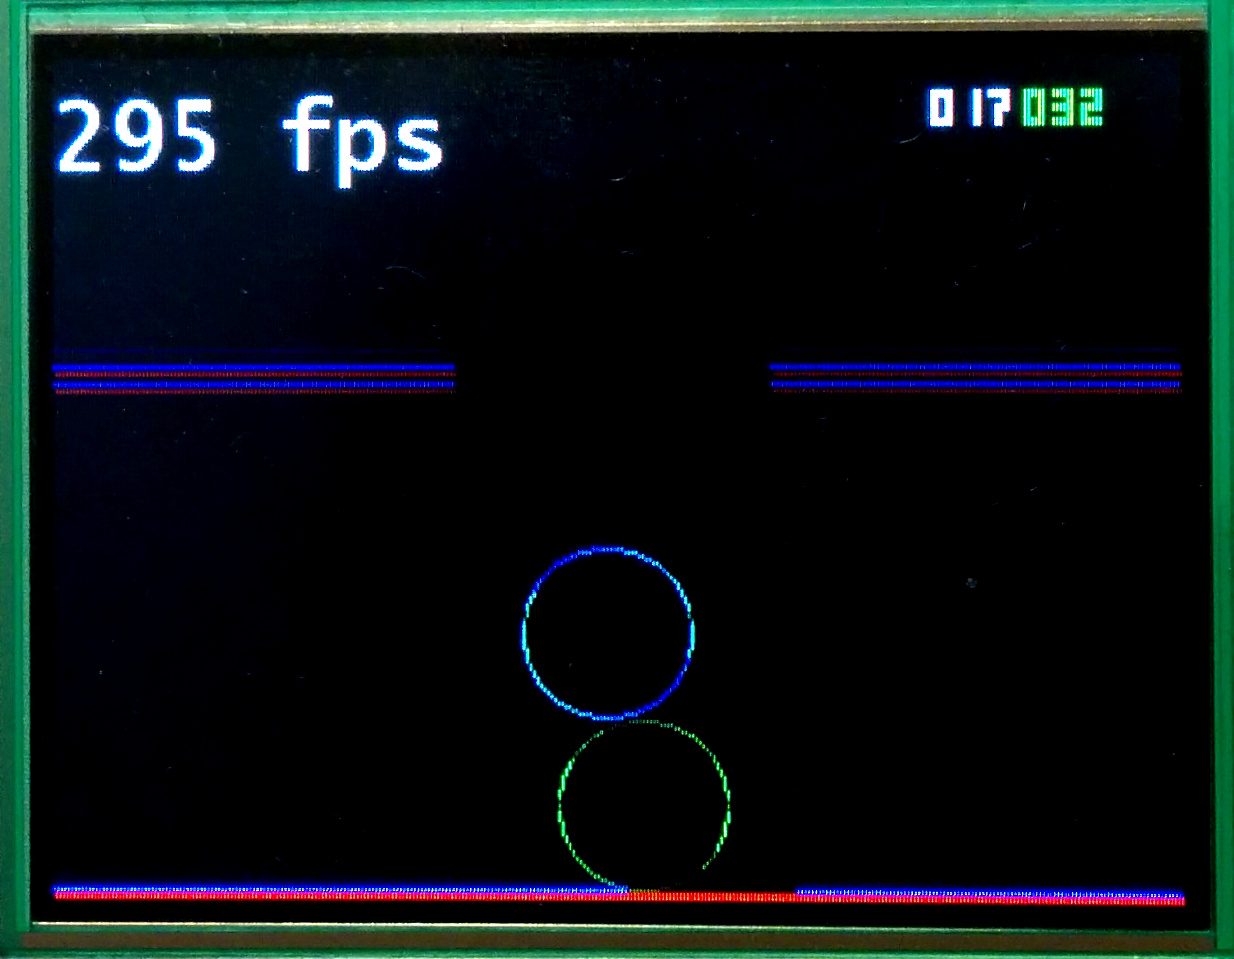
\includegraphics[width=0.5\textwidth]{figures/game-fps}
  \end{center}
  \caption{The on screen \gls{fps} on the {\DK}}
  \label{fig:res:fps}
\end{figure}


\subsection{Measurement Bias}
\label{sec:perf:bias}

When measuring performance, one has to consider a number of biases that can occur while performing the measurement.
A bias is an arbitrary external noise that might distort the result of the measurements.
Some of these biases can and should be eliminated before measuring, while others are harder or impossible to remove.

The following biases were found when analyzing the game application:
\begin{description}
  \item [User Input] \hfill \\
The game application was developed as a human playable game.
When measuring performance, deterministic results are preferable.
This bias was removed by implementing a simple deterministic artificial intelligence which emulates the user input.

  \item [Random Number Generator] \hfill \\
A \gls{rng} is used to generate a stream of seemingly random numbers.
To avoid performance impacts from the different \gls{rng} implementations for {\C} and {\rust,} a simple deterministic \gls{rng} was implemented and used.

  \item [Measurement Overhead] \hfill \\
Often when measuring the performance of an application at a course granularity, the measurement adds to the execution time.
This is largely the case when measuring \gls{fps}, as it adds profiling code to the actual application, thus affecting the performance of the application.
In this experiment, we are interested in the relative performance between {\C} code and {\rust} code.
Therefore, the added bias by the \gls{fps} measurement is acceptable as long as it is the same for both code bases.

  \item [Optimization Characteristics] \hfill \\
Various applications perform differently when subjected to different optimizations.
This fact leads to a trade-off when deciding the level of optimization to apply to the program.
To account for this bias, we look at the performance metric for all optimization levels.
\end{description}

\subsection{Results}
\label{sec:perf:res}

In this section, we present the results obtained when measuring performance.

\begin{figure}[H]
  \begin{center}
    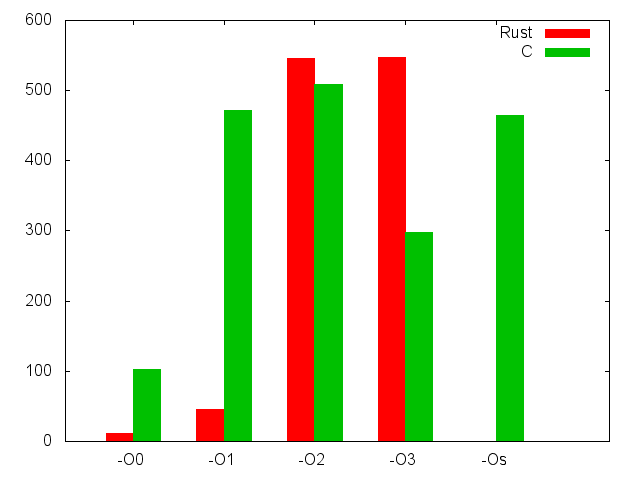
\includegraphics[scale=0.5]{results/plots/perf/perf.png}
  \end{center}
  \caption{Frame/Second achieved by {\rust} and {\C} code.}
  \label{fig:perf:res}
\end{figure}

\autoref{fig:perf:res} graphs the results for the performance measurements.
The Y-axis shows the number of Frames Per Seconds achieved by running the game on the optimization level given by the X axis.
We see that the {\C} code is \~10x faster on O0 and O1, but {\rust} equates by providing a 1.07x speedup over {\C} at O2.
C achieves the best performance at level O2 while {\rust} is slightly faster on O3 compared to O2.
Our brief analysis of this suggests that some of the high-level abstractions in {\rust} are fairly inefficient without optimizations.
An example of these abstractions is the \code{Iterator}-based \code{for} loop, which is used extensively throughout the {\cg} application.

The poor performance for the O3 optimization level for the {\C} was unexpected.
To further investigate this issue, we first considered the instruction cache hit ratio for the O3 and O2 binaries.
We did not find an explanation in the results, as the hit ratios were close to equal.

The optimization levels considered here, defines a set of individual optimizations which can be activated or deactivated by passing flags to the compiler.
Next we, looked at the change in performance due to each individual optimization flag in the set difference of $O3-O2$.
By adding each flag, one-by-one, from the set difference to an O2 base build, we managed to identify the source of the performance degradation.
The source was the \flag{-ftree-loop-distribute-patterns} flag.
This flag is used to collect common initializations of variables from different loop iterations and substitute these initializations with library routines like \lib{memset}.
We refer the reader to the \prog{gcc} documentation \cite{web:gcc} for further explanation of the flag.
The {\cg} application contains a fair amount of loops with initialization code, so if this optimization for our use-case is degrading the performance, it is quite natural for the overall performance to take a big hit.
For completeness; the performance of an O3 binary without the mentioned flag is equal in performance to the O2 binary for this application.


%The optimization Os for size is not available for {\rust} and is included for the discussion of size vs performance in \autoref{sec:res:size-v-perf}.
%\todo{I'm thinking there will be a larger discussion taking all the results in consideration in the end of this chapter}

%\subsection{Discussion}
%\label{sec:perf:disc}
%As \autoref{sec:perf:res} shows the performance of the application written in {\rust} not only matches the \gls{fps} performance of the {\C} version, it also provides a speedup of 1.07x.
%We also see that the optimizations are more predictable on this application in relation to optimization level, with perf(Ox) > perf(Oy) when x > y.
%This relationship does not hold for the {\C} application where the perf(O1) > perf(O3).
